\documentclass[conference,a4paper]{IEEEtran}
% IEEE conference two-column template. Compile: xelatex -> bibtex -> xelatex -> xelatex.
\usepackage{fontspec}
\setmainfont{Liberation Serif}
\setsansfont{Noto Sans}
\usepackage[turkish,shorthands=off]{babel}
\usepackage{amsmath,amssymb,booktabs,tabularx,array,makecell}
\usepackage{graphicx}
\usepackage[table]{xcolor}
\usepackage{tikz}
\usetikzlibrary{arrows.meta,positioning,shapes,calc}
\usepackage[hidelinks]{hyperref}
\usepackage{url}
\usepackage{microtype}
\usepackage{enumitem}
\usepackage{balance}
\setlist[itemize]{leftmargin=*,topsep=2pt,itemsep=1pt}
\setlist[enumerate]{leftmargin=*,topsep=2pt,itemsep=1pt}
\renewcommand\IEEEkeywordsname{Anahtar kelimeler}
\newcommand{\eng}[1]{\textit{#1}}
\newcommand{\code}[1]{\texttt{#1}}
\newcommand{\subpar}[1]{\par\noindent\textbf{#1}\quad}
\hypersetup{pdftitle={Dağıtık Görev Kuyruklarında Worker Arızaları ve Görev Kurtarma},pdfauthor={Emre Kurum}}
\title{Dağıtık Görev Kuyruklarında Worker Arızaları ve Görev Kurtarma:\\Celery--Redis Üzerinde Deneysel Bir Araştırma Tasarımı}
\author{\IEEEauthorblockN{Emre Kurum}
\IEEEauthorblockA{Bilgisayar Mühendisliği Tezli Yüksek Lisans\\
Süleyman Demirel Üniversitesi, Fen Bilimleri Enstitüsü\\
Öğrenci No: 2530138032\\
Dağıtık Sistemler --- 2026--2027 Güz\\
Ders sorumlusu: Doç. Dr. Asım Sinan Yüksel}}
\begin{document}
\maketitle
% Hoca vize için özet metninin boş bırakılmasını istedi.
\begin{abstract}
\mbox{}\vspace{0.7em}
\end{abstract}
\begin{IEEEkeywords}
dağıtık görev kuyrukları, işçi arızaları, hata toleransı, yeniden teslim, idempotency, Celery, Redis, PostgreSQL
\end{IEEEkeywords}

\section{Introduction (Giriş)}
Web uygulamalarında bazı işlemlerin kullanıcı isteği sırasında bitmesi beklenmez. Dosya işleme, rapor üretme veya toplu veri hazırlama gibi işler kuyruğa bırakılır; bir worker da uygun olduğunda işi alıp çalıştırır. API'nin hızlı yanıt vermesi açısından bu yöntem işe yarar. Fakat bir görevin kuyruğa alınması, onun sorunsuz biteceği anlamına gelmez. Worker aniden kapanabilir, broker ile bağlantısı kesilebilir veya veritabanına yazdığı sonucun ardından görev tamamlandı bilgisini gönderemeyebilir.

Beni bu konuda özellikle ilgilendiren durum, \emph{veritabanına kayıt yazıldıktan hemen sonra} worker'ın kapanmasıdır. Örneğin bir belge işleme görevi PostgreSQL'de sonuç satırını oluşturmuş, fakat Redis üzerinden yürütülen görevin onayını henüz tamamlayamamış olabilir. Mesaj yeniden işlenirse ikinci bir worker aynı işi tekrar çalıştırabilir. Tersi de mümkündür: görev erkenden onaylanmış, fakat kayıt oluşmadan worker durmuşsa kullanıcı işi eksik kalabilir. Bu iki durumun aynı ``görev başarısız'' etiketi altında görülmesi, hatanın nedenini anlamayı zorlaştırır.

Kuyruk sisteminde yeniden teslim edilen \emph{mesaj} ile veritabanında oluşan \emph{iş sonucu} farklı şeylerdir. \eng{Retry} bir işlemi yeniden denemeyi sağlar. \eng{Idempotency} ise aynı mantıksal işlem tekrar denense bile ikinci bir kalıcı etki oluşturmamayı hedefler. Bunları iki rakip yöntem olarak karşılaştırmak doğru olmaz; birlikte kullanıldıklarında nasıl davrandıklarını incelemek daha anlamlıdır. Güncel çalışmalar da tekrar çalıştırma sırasında paylaşılan durumun bozulabileceğini ve hata durumunun ayrıca test edilmesi gerektiğini gösteriyor~\cite{stoica2024,ding2023,qi2023}.

Kendi yazılım projelerimde Celery ve Redis'i arka plan işlemleri için kullandım. Bu nedenle çalışmayı bildiğim bir mimari üzerinden kurmak istiyorum. Araştırma sorusunu çok geniş tutmak yerine şu duruma odaklanıyorum: \textbf{İki bağımsız worker'dan biri görev sırasında kapanırsa, diğer worker aynı işi devralabiliyor mu ve veritabanındaki sonuç doğru kalıyor mu?} Yanıtı, yalnızca kuyruk durumuna bakarak değil worker günlükleriyle PostgreSQL kayıtlarını birlikte inceleyerek arayacağım.

\subsection{Çalışmanın kapsamı}
Planlanan ortamda bir görev üretici, Redis broker, Worker A, Worker B ve PostgreSQL yer alıyor. Worker'lar ayrı konteynerlerde çalışacak ve aynı kuyruktan ağ üzerinden görev alacak. Worker A belirlenmiş bir aşamada durdurulurken diğer bileşenler çalışmaya devam edecek. Böylece yarım kalan veya onayı tamamlanmayan işin Worker B tarafından alınıp alınmadığını ölçmek mümkün olacak. Çalışma, tüm mesajlaşma ürünlerini ya da internet üzerindeki çok bölgeli sistemleri karşılaştırmayı amaçlamıyor. İlk deneyler aynı bilgisayarda kurulan ayrı konteynerlerle sınırlı olacak.

Bu vize raporunda problem, ilgili yayınlar, araştırma soruları ve deney yöntemi ele alınıyor. Ölçüme dayalı sonuçlar ancak prototip kurulduktan sonra yazılabilir; bu nedenle sonuç, tartışma ve kapanış başlıkları bu aşamada boş bırakılmıştır.

\section{Related Work (Literatür Taraması)}
Bu bölümde yalnızca aynı teknolojiyi kullanan yayınlar değil, konumuzla ilişkili üç araştırma alanı incelenmiştir: tekrar yürütmede doğru sonuç üretme, dağıtık sistemlerde arızayı sistematik olarak tetikleme ve farklı bileşenler arasında veri tutarlılığı. Kaynaklar 2021--2026 arasında uluslararası konferans veya dergilerde yayımlanmış çalışmalardan seçilmiştir. Bunların tümünün Celery'yi doğrudan ele aldığı iddia edilmemektedir; her yayının çalışmaya katkısı ayrı belirtilmiştir.

\subsection{Yeniden deneme ve idempotent işlem yürütme}
Stoica ve arkadaşları, gerçek yazılımlardaki retry hatalarının hem kaynak kodunda hem de testlerde yakalanmasının neden zor olduğunu inceler. SOSP 2024'te yayımlanan bu çalışma, bir işlemin tekrar denenmesinin basit bir hata yakalama bloğuna indirgenemeyeceğini gösterir~\cite{stoica2024}. Bir görev tekrar çalıştığında dış sisteme daha önce yazılmış verinin nasıl yorumlanacağı ayrıca ele alınmalıdır. Planlanan deneyde bu düşünce, görev denemesinin kendisi ile PostgreSQL üzerinde oluşan nihai kaydı ayrı ölçme kararını destekler.

Ding ve arkadaşlarının OSDI 2023'te sunduğu Flux, durumlu sunucusuz fonksiyonlarda idempotence özelliğini doğrulamaya yöneliktir~\cite{ding2023}. Çalışma, hata sonrası fonksiyonun yeniden çalışmasının paylaşılan durumda tutarsızlık yaratabileceğini gösterir; otomatik doğrulama yoluyla sorunlu işlemleri bulmaya çalışır. Bu yayın Celery'yi incelemese de tekrarlanan yürütmenin uygulamanın kullanıcıya görünen sonucu açısından değerlendirilmesi gerektiğini açıklar. Bu çalışmada ise resmî doğrulama yerine kontrollü bir PostgreSQL kaydı ve olay günlüğü kullanılacaktır.

Qi ve arkadaşlarının Halfmoon sistemi, durumlu serverless fonksiyonlarda hata toleransının loglama maliyetini inceler~\cite{qi2023}. Aynı araştırma çizgisinin 2025 tarihli dergi çalışması, asimetrik loglama ile doğru yeniden yürütme ve performans maliyeti arasındaki ilişkiyi daha kapsamlı ele alır~\cite{qi2025}. Bu iki yayın yeni bir görev kuyruğu sunmak yerine uygulama durumunu doğru korumaya odaklanır. Celery üzerindeki basit prototipimizin bu sistemlerle aynı güvenceyi verdiği iddia edilmeyecek; yalnızca bir arıza sonrası tekrarın kalıcı veri etkisini nasıl değiştirdiğini incelemede kavramsal dayanak sağlayacaklardır.

Psarakis ve arkadaşlarının EDBT 2024 çalışması, durumlu uygulama bileşenlerini dağıtık veri akışları olarak yürütmeyi ve altta yatan motorun işlem garantilerini uygulama modelinden ayırmayı tartışır~\cite{psarakis2024}. Bu yaklaşım, mesaj aktarım mekanizmasıyla uygulamanın kalıcı yazmasının aynı işlem sınırında bulunmadığını hatırlatır. Önerilen prototipde Redis ile PostgreSQL arasında ortak bir atomik işlem kurulmayacaktır. Bu nedenle uygulama tarafında benzersiz işlem anahtarının nasıl kullanılacağı araştırmanın merkezindedir.

\subsection{Arıza enjeksiyonu ve deneylerin yeniden üretimi}
Meiklejohn ve arkadaşlarının SoCC 2021 çalışması, servis bağımlılıkları arasındaki kısmi arızaları sistematik olarak test etmeyi hedefleyen \eng{Service-Level Fault Injection Testing} (SFIT) yöntemini ve Filibuster aracını tanıtır~\cite{meiklejohn2021}. Çalışmanın temel katkısı, üretimde gerçekleşmesini beklemek yerine belirli arıza noktalarının test ortamında oluşturulabilmesidir. Planlanan deneyde de işçi sonlandırmasını rastgele değil, kayıt öncesi ve kayıt sonrası gibi tanımlanmış aşamalarda uygulamak bu fikirle uyumludur.

Assad ve arkadaşları, ICSE 2024'te mikroservislerin güvenilmez bir veritabanına karşı davranışını sınamaya odaklanmıştır~\cite{assad2024}. Bu çalışma, yalnızca servisler arası çağrıların değil kalıcı depolama bağımlılıklarının da arıza senaryolarında önemli olduğunu gösterir. Veritabanının hata vermesi, worker'ın veritabanına başarıyla yazdıktan sonra kapanmasıyla aynı durum değildir. Çalışma bu ayrımı açık tutacak ve ilk aşamada PostgreSQL hizmetini çalışır bırakıp yalnızca işçi arızasını enjekte edecektir.

Gao ve arkadaşlarının ICSE 2023'teki CrashFuzz araştırması, düğüm çökmesi ve yeniden başlatma kombinasyonlarıyla ortaya çıkan toparlanma hatalarını kapsam güdümlü biçimde arar~\cite{gao2023}. Feng ve arkadaşlarının ICSE 2024'te sunduğu FaultFuzz ise dağıtık sistemlerde çalışma zamanı geri bildiriminden faydalanarak hata enjeksiyonunu yönlendirir~\cite{feng2024}. Bu iki çalışmanın test ettiği altyapıların doğrudan Celery olmadığı önemlidir. Buradaki yöntemsel katkı, "arıza oldu" demek yerine arızanın sırası, türü ve gerçekleştiği durumun kaydını tutmaktır.

Wu, Pan ve Huang'ın NSDI 2024'te sunduğu Legolas, kısmi hizmet arızalarını ortaya çıkarmak için soyut durumlara göre enjeksiyon noktası seçer~\cite{wu2024}. Pan ve arkadaşlarının SOSP 2024 tarihli Anduril çalışması ise bir arızayı yeniden üretirken doğru hata türü ve zamanlamasını bulmanın önemini araştırır~\cite{pan2024}. Bu makalelerden, ölçümün yeniden üretilebilir olması için gözlemlenebilir olay sırası gerektiği sonucu çıkarılabilir. Bizim düzenimizde bu olaylar worker'ın görevi alması, PostgreSQL'in commit etmesi, worker'ın kapatılması ve olası yeniden teslim şeklinde kaydedilecektir.

Chen ve arkadaşlarının \eng{MicroFI} çalışması, mikroservislerde istek düzeyinde kontrollü hata enjeksiyonunu ve önemli hata noktalarının seçilmesini ele alır~\cite{chen2024}. Ahmad ve arkadaşları ise 2024 tarihli dergi çalışmalarında farklı kullanıcı yükleri ve gecikme enjeksiyonlarının bulut uygulamalarındaki performans ve erişilebilirlik üzerindeki etkilerini inceler~\cite{ahmad2024}. Bizim deneyin iş yükü bu yayınlarla aynı değildir; yine de arızasız temel koşulu, eşit yükleri ve kontrollü tekrarları kullanmak karşılaştırma açısından gereklidir.

Naqvi ve arkadaşlarının ACSOS 2022 çalışması, kendi durumunu onarmaya çalışan sistemlerin yalnızca çalışır görünmesinin yeterli olmadığını, beklenmedik koşullara verdiği tepkinin ayrıca sınanması gerektiğini tartışır~\cite{naqvi2022}. Poltronieri ve arkadaşları da NOMS 2022'de kaos mühendisliği deneylerini servis yapılandırmalarının dayanıklılığını değerlendirmek için kullanmıştır~\cite{poltronieri2022}. Her iki çalışmada da arızasız ölçüm ile arızalı ölçümün karşılaştırılabilmesi için test koşullarının önceden belirlenmesi önemlidir. Planlanan deney bu araştırmalardan çok daha küçük ölçekli olsa da aynı gerekçeyle başlangıç durumunu, enjeksiyon zamanını ve değiştirilen ayarı kayıt altına alacaktır.

Feng ve arkadaşlarının ICSE 2025'te yayımladığı REDII, dağıtık sistemlerde hatanın deterministik biçimde yeniden oluşturulmasını destekleyen bir test altyapısı sunar~\cite{feng2025}. Bu çalışmadan alınacak temel yöntemsel ders, arızanın yalnızca rastlantısal olarak üretilmesi değil deney koşulunun yeniden çalıştırılabilir olmasıdır. Çalışmada düzenlenmiş görev kimlikleri, sürümleri sabitlenmiş konteynerler ve arıza komutlarının zaman damgaları kullanılacaktır.

\subsection{Bileşenler arası tutarlılık}
Loff ve arkadaşlarının SOSP 2023 tarihli Antipode araştırması, farklı veri depolarını kullanan servisler arasındaki nedensel tutarlılığın korunmasını ele alır~\cite{loff2023}. İncelenen sorun Celery task ACK'siyle aynı değildir; ancak servis ve veri depolarının farklı durum bilgilerini taşıması nedeniyle uygulamanın bütünsel davranışının tek bir servis kaydından anlaşılamayacağını gösterir. Bu nedenle hem broker hem de veritabanı olayları ayrı kaydedilerek raporlanacaktır.

\subsection{Literatürden çıkan araştırma boşluğu}
Yukarıdaki yayınlar retry hatalarının tespiti, idempotence doğrulaması, serverless durum yönetimi, hata enjeksiyonu ve tutarlılıkla ilgili güçlü sonuçlar sunuyor. Bununla birlikte bu çalışmaların her biri farklı çalışma ortamları, arıza modelleri ve ölçüm düzeyleri kullanıyor. Bizim ders çalışması açısından sınanabilir boşluk, aynı Celery--Redis--PostgreSQL kurulumunda şu üç etkiyi bir arada görünür hâle getirmektir: \textbf{ACK zamanlaması}, \textbf{worker kaybı sonrası yeniden teslim} ve \textbf{aynı kalıcı kaydın iki kez yazılmasını önleme}. Bu özel deney matrisinin alan literatüründe ilk kez önerildiği iddia edilmemektedir. Önerilen katkı yeni bir algoritma bulmaktan çok, bilinen mekanizmaların hangi arıza aşamasında ne sonuç verdiğini tekrarlanabilir bir örnekte karşılaştırmaktır.

\begin{table*}[t]
\caption{Seçilmiş güncel yayınların araştırma sorumuz açısından karşılaştırılması. Çalışmaların uygulama ortamları farklıdır; tablo doğrudan performans karşılaştırması değildir.}
\centering\footnotesize
\begin{tabularx}{\textwidth}{@{}p{29mm}p{42mm}p{43mm}X@{}}
\toprule
\textbf{Çalışma} & \textbf{Odak noktası} & \textbf{Bizim çalışmada kullanılacak yönü} & \textbf{Doğrudan kapsamadığı boyut}\\
\midrule
Stoica vd. (2024)~\cite{stoica2024} & Gerçek sistemlerde retry hataları & Tekrar çalıştırılan işin yan etkisinin izlenmesi & İki Celery worker'ıyla görev devri\\
Ding vd. (2023)~\cite{ding2023} & Durumlu fonksiyonlarda idempotence doğrulama & Yeniden denemede kullanıcıya görünen iş etkisi & Redis visibility timeout / ACK penceresi\\
Qi vd. (2023, 2025)~\cite{qi2023,qi2025} & Loglamalı hata toleranslı serverless yürütme & Durum tutarlılığı ve maliyet ayrımı & PostgreSQL \code{ON CONFLICT} deneyi\\
Meiklejohn vd. (2021)~\cite{meiklejohn2021} & Servis düzeyi hata enjeksiyonu & Arıza aşamasının kontrol edilmesi & İşçi özelinde ACK semantiği\\
Assad vd. (2024)~\cite{assad2024} & Veritabanı bağımlılığında dayanıklılık & DB işleme aşamasının ayrı gözlenmesi & Celery task redelivery koşulları\\
Gao vd. (2023), Wu vd. (2024)~\cite{gao2023,wu2024} & Çökme ve kısmi arızaların aranması & Arıza sırası ve güvenilir tekrar & Göreve özel idempotency anahtarı\\
Pan vd. (2024), Feng vd. (2025)~\cite{pan2024,feng2025} & Hataların deterministik yeniden üretimi & Olay günlüğü, tekrarlanan deney & İki işçiyle basit iş devri matrisi\\
\bottomrule
\end{tabularx}
\label{tab:literature}
\end{table*}

\subsection{Bu çalışmaların bizim deneye bıraktığı sorular}
Flux ve Halfmoon tekrar çalıştırma sırasında verinin bozulmaması için daha kapsamlı yöntemler geliştiriyor~\cite{ding2023,qi2023,qi2025}. CrashFuzz, Legolas, Anduril ve REDII ise arızaların hangi sırada ortaya çıktığını bulmaya veya aynı koşulları yeniden oluşturmaya çalışıyor~\cite{gao2023,wu2024,pan2024,feng2025}. Bu yayınların kullandığı araçlar ve ölçekler birbirinden farklı. Burada aynı sistemleri yeniden geliştirmeye çalışmak yerine, daha küçük bir Celery--Redis deneyinde onların işaret ettiği sorunları görünür kılmak hedefleniyor.

Araştırmada dört ayrı bilgi toplanacak: \textbf{(i)}\ görevin broker tarafından teslim edilmesi, \textbf{(ii)}\ işi hangi worker'ın ne zaman başlattığı, \textbf{(iii)}\ PostgreSQL kaydının gerçekten commit edilmesi ve \textbf{(iv)}\ görevin yeniden teslim edilip edilmediği. Bunlar tek olay değildir. Özellikle Worker B'nin yeni bir işi tamamlaması, Worker A'daki yarım kalan işi devraldığını kanıtlamaz. Devir sayılabilmesi için aynı mantıksal iş kimliğinin iki worker'ın kayıtlarında görülmesi gerekir.

Bir başka sınır da \code{task\_id} ile \code{operation\_id} farkıdır. İlk değer Celery'nin teknik görev kimliğidir; ikincisi veritabanına yazılmasını beklediğimiz işin kimliğidir. Bir iş yeniden yayımlanırsa teknik görev kimliği değişebilir. Bu nedenle çift iş etkisini teknik mesaj sayısına bakarak değil, \code{operation\_id} başına oluşan nihai kayıt sayısıyla ölçeceğiz. Bu tercih, idempotence araştırmalarında vurgulanan kullanıcıya görünen sonuçla da uyumludur~\cite{ding2023,stoica2024}.

\subsection{Literatür ve deney arasındaki sınır}
Seçilen yayınların çoğu Celery'ye özel değildir. Bir bölümü durumlu sunucusuz fonksiyonları, bir bölümü büyük dağıtık sistemleri veya mikroservis arızalarını inceler. Bu yayınlardan doğrudan ``Celery'de şu ayar daha hızlıdır'' gibi bir sonuç çıkarılamaz. Onlardan yararlandığımız yer, hangi arızayı nasıl oluşturacağımız ve hangi çıktıyı ölçmemiz gerektiğidir. Celery'nin gerçek ACK davranışı için resmî görev ve Redis belgeleri ayrıca kullanılacaktır~\cite{celerytasks,celeryredis}. Böylece araştırma makalelerinden gelen çıkarımla bir ürünün yapılandırma bilgisini birbirine karıştırmamış olacağız.

Bu araştırmanın katkısı, yeni bir kuyruk algoritması önermek değil; bilinen mekanizmaların aynı iki-worker ortamında, aynı arıza anlarında ve aynı veritabanı işlemi üzerinde nasıl davrandığını göstermek olacak. Ölçüm sonunda bazı konfigürasyonlar arasında fark çıkmayabilir. Bu da geçerli bir bulgudur. Önemli olan işlemin hangi aşamada durduğu ve sonuçta kayıp ya da çift kayıt oluşup oluşmadığının izlenebilmesidir.

\section{Research Questions (Araştırma Soruları)}
Araştırmanın temel sorusu şu şekilde belirlenmiştir: \textit{Aynı Redis broker'ına ağ üzerinden bağlanan iki bağımsız Celery işçisinden biri, PostgreSQL'e yazmadan önce veya yazdıktan sonra beklenmedik şekilde kapanırsa; mesajın başka işçiye teslimi ve tek bir kalıcı iş etkisi hangi ACK, worker-loss ve idempotency yapılandırmalarında sağlanabilir?}

Bu soruyu daha net ölçebilmek için dört alt soruya ayırdım:
\begin{enumerate}
\item \textbf{AS1 -- Görevin devri:} Worker A arızalandığında Worker B görevi devralabiliyor mu? Erken onay, geç onay ve kayıp işçi ayarları sonucu nasıl etkiliyor?
\item \textbf{AS2 -- Çift işleme:} Worker A PostgreSQL'e yazıp ACK öncesinde kapanırsa birden fazla yürütme denemesi ve birden fazla kalıcı kayıt oluşuyor mu?
\item \textbf{AS3 -- Idempotency:} PostgreSQL üzerinde atomik işlem anahtarı kullanmak, yeniden yürütmenin oluşturabileceği yinelenen kalıcı sonucu engelliyor mu? Bu kontrolün gecikme maliyeti nedir?
\item \textbf{AS4 -- Arıza türü:} Worker çocuk sürecinin kapanması ile worker konteynerinin bütünüyle durmasının yeniden teslim ve kurtarma süresi üzerindeki etkileri aynı mı?
\end{enumerate}

\subsection{Ön hipotezler}
\textbf{H1:} Belirli işçi kaybı türlerinde geç ACK ve uygun yeniden teslim seçenekleri, görevin başka bir worker tarafından tamamlanma olasılığını artırır. Bunun her tür arıza için geçerli olduğu peşinen varsayılmayacaktır. \textbf{H2:} Aynı iş birden fazla kez yürütülse de benzersiz \code{operation\_id} kısıtı ile atomik yazma kullanılması, tek veritabanındaki çift kalıcı kayıtları önler. \textbf{H3:} Arıza sonrası kurtarmanın süresi, Redis'in visibility timeout ve worker-loss davranışından etkilenebilir. \textbf{H4:} Uygulama düzeyindeki retry ayarının etkisini, broker kaynaklı yeniden teslimden ayrı bir deneyde ölçmek gerekir.

Hipotezler ölçüm sonucu değildir. Özellikle Celery'nin geç ACK seçeneği, işçi çocuk süreci öldüğünde bazı durumlarda yeniden teslimi otomatik sağlamaz. Resmî görev kılavuzundaki \code{task\_reject\_on\_worker\_lost} davranışı ve Redis üzerindeki \code{visibility\_timeout} bu nedenle deneyin açık değişkenleri olacaktır~\cite{celerytasks,celeryredis}.

\section{Method (Yöntem)}
\subsection{Deney düzeneği ve çalıştırma ortamı}
Kontrollü, tekrarlanabilir bir prototip deneyi planlanmıştır. Prototipte görev üretici bir Python API servisi, ortak Redis broker, ayrı konteynerlerde çalışan iki Celery işçisi ve kalıcı kayıtların tutulduğu PostgreSQL olacaktır. Worker A ve Worker B aynı görev türünü dinleyecek ancak birbirlerinin belleğini paylaşmayacak. İletişim yalnızca ağ üzerinden Redis ve PostgreSQL bağlantılarıyla gerçekleşecektir. Arıza enjekte edildiğinde yalnızca Worker A durdurulacak; Worker B, broker ve veritabanı çalışır kalacaktır. Böylece işin başka bir işçiye aktarılması gerçekten test edilebilecektir.

\begin{figure}[t]
\centering
\resizebox{\columnwidth}{!}{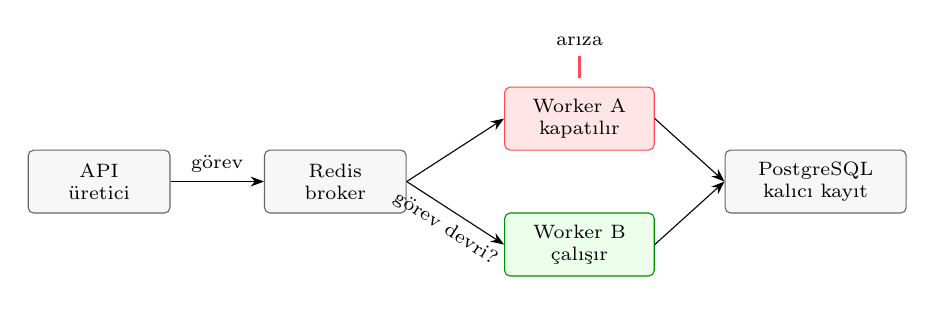
\begin{tikzpicture}[>=Stealth,font=\scriptsize,
  nodebox/.style={draw=black!60,rounded corners=2pt,align=center,minimum height=8mm,fill=black!3},
  fault/.style={nodebox,fill=red!10,draw=red!70},
  live/.style={nodebox,fill=green!8,draw=green!55!black}]
\node[nodebox,minimum width=18mm] (api) at (0,0) {API\\üretici};
\node[nodebox,minimum width=18mm] (redis) at (3.0,0) {Redis\\broker};
\node[fault,minimum width=19mm] (wa) at (6.1,.80) {Worker A\\kapatılır};
\node[live,minimum width=19mm] (wb) at (6.1,-.80) {Worker B\\çalışır};
\node[nodebox,minimum width=23mm] (pg) at (9.1,0) {PostgreSQL\\kalıcı kayıt};
\draw[->] (api) -- node[above]{görev} (redis);
\draw[->] (redis.east) -- (wa.west);
\draw[->] (redis.east) -- node[below,sloped]{görev devri?} (wb.west);
\draw[->] (wa.east) -- (pg.west);
\draw[->] (wb.east) -- (pg.west);
\draw[red!70,thick] (6.10,1.32)--(6.10,1.60) node[above,black]{\scriptsize arıza};
\end{tikzpicture}
}
\caption{Planlanan dağıtık prototip: iki bağımsız worker ortak broker'a ağ üzerinden bağlıdır. Kırmızı bileşene kasıtlı arıza uygulanır.}
\label{fig:arch}
\end{figure}

Her görev, \code{operation\_id} adlı sabit bir mantıksal işlem kimliğiyle yayımlanacaktır. Celery'nin \code{task\_id} değeri ayrıca saklanır. Bunların farklı kavramlar olması önemlidir: görevin yeniden yayımlanması teknik görev kimliğini değiştirebilir, fakat uygulamanın iş kimliği aynı kalmalıdır. Görev çalışırken worker kimliği, deneme sırası, başlama saati, kayıt öncesi aşama, commit tamamlanması ve görev bitişi ayrı olaylar olarak izlenecektir. Arıza komutunu tetikleyen test yürütücüsü de bağımsız olay günlüğü tutacaktır.

İlk denemeler tek bilgisayardaki Docker konteynerleriyle yapılacaktır. Bu düzen gerçek dağıtık iletişimi içermekle birlikte bağımsız fiziksel makine arızalarının tamamını temsil etmez. Özellikle ana bilgisayarın bütünüyle kapanması, Redis'in arızalanması ve ağ bölünmesi ana deneyin dışında tutulur. Yöntem, bu sınır açıkça belirtilerek raporlanacaktır.

\subsection{Kalıcı verinin oluşturulması}
Temel görev, küçük bir simüle belge işleme sonucu olarak tek satırlık kayıt oluşturacaktır. Başarılı iş etkisi, \code{operations} tablosunda beklenen \code{operation\_id} için bir satırın kalıcı olarak yazılmasıdır. İdempotency kapalı koşulda aynı mantıksal işlem tekrarlandığında ayrı fiziksel satırların oluşması mümkün bırakılacaktır. İdempotency açık koşulda \code{operation\_id} için benzersiz kısıt tanımlanacak ve \code{INSERT ... ON CONFLICT} benzeri atomik kayıt stratejisi kullanılacaktır~\cite{postgresunique}. Kayıt denetiminin ayrı bir SELECT işlemiyle yapılıp sonradan INSERT çalıştırılması yeterli görülmez; bu yöntem iki worker eşzamanlı çalıştığında yarış koşulu oluşturabilir.

Tabloda \code{operation\_id}, \code{created\_at}, \code{worker\_id}, \code{attempt\_id} ve sonuç hash'i gibi alanlar bulunacaktır. Deneme günlüğü ayrı tabloda tutulacak; idempotency açık koşulda bir görev tekrar çalışsa bile girişimlerin hepsi gözlenebilecek ancak nihai iş kaydı tekil kalabilecektir. Bu, "görev birden fazla kez çalıştı" ile "kullanıcının işi iki kez yapıldı" ifadelerini karıştırmamayı sağlayacaktır.

\subsection{ACK, retry ve yeniden teslimin ayrılması}
Celery'de erken ACK etkinse, broker görevi işlenmeden önce onaylanmış sayabilir. Geç ACK kullanımında görev tamamlandıktan sonra onaylanması hedeflenir. Bununla birlikte \code{acks\_late=True}, çocuk işçi sürecinin beklenmedik ölümü halinde otomatik olarak "mutlaka yeniden teslim" anlamına gelmez. Celery belgelerindeki worker-loss seçenekleri ayrıca uygulanacaktır~\cite{celerytasks}. Redis broker'ın visibility timeout süresi de kapanan işçiye ait görevin ne zaman yeniden görünür olacağını değiştirebilir~\cite{celeryredis}.

Ölçümün birinci aşamasında uygulama düzeyindeki \code{retry()} ve \eng{autoretry} kapatılacaktır. Böylece bir görev ikinci kez başlatılırsa bunun geçici Python hatasından değil broker/worker davranışından kaynaklandığı anlaşılabilir. İkinci aşamada yalnızca geçici hata üreten görevler seçilerek retry sayısı ve gecikme politikası ayrıca test edilecektir. Bu iki aşama aynı tabloda alternatif algoritmalar gibi sunulmayacaktır.

\begin{table}[t]
\caption{Ana deneyin yapılandırma grupları (planlanan karşılaştırma).}
\centering\footnotesize
\begin{tabularx}{\columnwidth}{@{}p{8mm}p{19mm}X@{}}
\toprule
Kod & ACK / worker loss & Veritabanında kayıt yöntemi\\
\midrule
K0 & Erken ACK & Idempotency yok\\
K1 & Geç ACK, worker-loss reject kapalı & Idempotency yok\\
K2 & Geç ACK, worker-loss reject açık & Idempotency yok\\
K3 & K2 ile aynı & Atomik idempotency açık\\
K4 & K1 ile aynı & Atomik idempotency açık\\
\bottomrule
\end{tabularx}
\label{tab:configs}
\end{table}

K0--K4 yapılandırmaları sırayla ve birbirinden bağımsız olarak çalıştırılacaktır. Uygulama ve veritabanı aynı sürümle kullanılacak; her tekrar öncesinde test kayıtları temizlenecektir. Redis anahtarları da deneyin sonucunu taşıyan beklemedeki görevleri yanlışlıkla silmeyecek biçimde sıfırlanacaktır. Böylece önceki denemeden kalan mesajlar yeni deneyin sonucu gibi kaydedilmeyecektir.

\subsection{Arıza senaryoları ve doğru zamanda sonlandırma}
Dört temel senaryo uygulanacaktır. \textbf{S0} arızasız durumda görevin normal tamamlanmasıdır. \textbf{S1} PostgreSQL kaydından önce Worker A'nın sonlandırılmasıdır. \textbf{S2} PostgreSQL commit tamamlandıktan sonra fakat Celery ACK onayından önce Worker A'nın sonlandırılmasıdır. \textbf{S3} Worker A arızasından sonra Worker B'nin görevi devralıp devralamadığının uzun bir izleme penceresiyle incelenmesidir. S3, S1 ve S2'nin daha ayrıntılı izlenen bir devam koşulu olarak kullanılabilir; ayrı bir bağımsız arıza türü olarak raporlanmayacaktır.

\begin{figure}[t]
\centering
\resizebox{\columnwidth}{!}{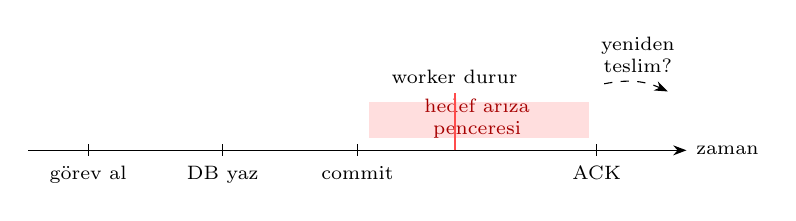
\begin{tikzpicture}[>=Stealth, font=\scriptsize, x=0.95cm,y=.65cm]
\draw[->] (0,0) -- (8.8,0) node[right]{zaman};
\foreach \x/\label in {0.8/{görev al},2.6/{DB yaz},4.4/{commit},7.6/{ACK}}{
 \draw (\x,.12)--(\x,-.12);
 \node[align=center,below] at (\x,-.12) {\label};
}
\fill[red!13] (4.55,.25) rectangle (7.5,.95);
\node[align=center,red!65!black] at (6.0,.62) {hedef arıza\\penceresi};
\draw[red!70,thick] (5.70,0)--(5.70,1.12);
\node[above] at (5.70,1.12){worker durur};
\draw[->,dashed] (7.7,1.30) to[bend left=18] (8.55,1.15);
\node[above,align=center] at (8.15,1.33) {yeniden\\teslim?};
\end{tikzpicture}
}
\caption{Kalıcı kayıt ile ACK arasında hedeflenen arıza penceresi. İşaretlenen aralığın gerçekten yakalandığı olay günlüğüyle doğrulanacaktır.}
\label{fig:timeline}
\end{figure}

Arıza enjeksiyonunun hedeflenen noktada uygulanabilmesi için görev içine yalnızca deney ortamında açılan senkronizasyon kancaları eklenecektir. İşçi \code{before\_commit} veya \code{after\_commit} aşamasına geldiğinde test yürütücüsü olayın kaydını alıp ilgili işçi sürecini durduracaktır. Arıza penceresinin tam olarak yakalandığı varsayılmaz; PostgreSQL commit kaydı, uygulama olayı ve worker kapatma zamanı karşılaştırılacaktır. Eğer işçi ACK'yi çoktan göndermişse koşul başarısız hata enjeksiyonu olarak işaretlenerek ana sonuç grubuna dahil edilmeyecektir.

Her senaryo iki sonlandırma biçimiyle denenmelidir: \textbf{F1}, Celery'nin görev çalıştıran çocuk sürecinin kapatılması; \textbf{F2}, Worker A konteynerinin tümden durdurulması. Bu ayrım zorunludur çünkü işçi süreci kaybıyla tüm konteynerin broker bağlantısını yitirmesi Celery açısından aynı durum değildir. Amaç sonuçları önceden tahmin etmek değil bu davranış farkının gözlenip gözlenmediğini sınamaktır.

\begin{table}[t]
\caption{Hata enjeksiyonu koşulları ve beklenen gözlemler.}
\centering\footnotesize
\begin{tabularx}{\columnwidth}{@{}p{8mm}p{31mm}X@{}}
\toprule
Kod & Enjeksiyon yeri & Kontrol edilen olay\\
\midrule
S0 & Arıza yok & Tek iş etkisi ve normal süre\\
S1 & Commit öncesi & İş kaybı, yeniden teslim, Worker B\\
S2 & Commit sonrası / ACK öncesi & Tekrar deneme ve çift kayıt\\
F1 & Çocuk işçi süreci kapalı & Worker-loss ayarı davranışı\\
F2 & Worker A konteyneri kapalı & Broker bağlantısı sonrası devralma\\
\bottomrule
\end{tabularx}
\label{tab:faults}
\end{table}

\subsection{Deney adımları}
Deney planı küçük adımlara bölünmüştür. Önce arızasız sistemde Worker A ile Worker B'nin ayrı işlem kimliklerine ve ağ bağlantılarına sahip olduğu doğrulanacaktır. İkinci adımda beklenen iş kaydının ne zaman oluştuğu ve normal gecikmenin dağılımı ölçülecektir. Üçüncü adımda küçük bir görev grubu için arıza enjeksiyonu çalıştırılarak hedeflenen commit öncesi/sonrası ayrımının günlüklerden okunabildiği kontrol edilecektir. Bundan sonra yapılandırma matrisiyle tekrarlar başlatılacaktır.

Her deney grubunun başlangıcında aynı sayıdaki mantıksal görev üretilir, aynı yapay işleme gecikmesi uygulanır ve Worker A'nın hedeflenen görevleri aldığı doğrulanır. Sadece gerekli konfigürasyon değişkeni değiştirilir. İlk pilot için her koşulda 50 görev ve 3 tekrar yeterli bir hata ayıklama başlangıcı olabilir; bu sayı bilimsel sonuç çıkarmak için önceden yeterli ilan edilmez. Pilot sonrasında zaman ve bilgisayar kaynakları uygunsa koşul başına 300--500 görev ve en az beş bağımsız tekrar hedeflenir. Ana deneyin büyüklüğü gözlenen varyans ve ölçümlerin kararlılığına göre kesinleştirilecektir.

\subsection{Ölçümler}
\textbf{Tamamlanan mantıksal görev oranı}, belirlenen izleme penceresi içinde beklenen kalıcı iş etkisini oluşturan benzersiz \code{operation\_id} sayısının toplam görev sayısına oranıdır. \textbf{Çoklu deneme oranı}, aynı mantıksal işin birden fazla girişim günlüğüne sahip olmasıdır. \textbf{Çift iş etkisi oranı}, aynı mantıksal iş için birden fazla kalıcı sonuç oluşmasıdır. Bu son ölçümün idempotency açık durumda benzersizlik kısıtı tarafından engellenmesi beklenir; fakat veritabanı kontrolü dışındaki etkiler için aynı garanti iddia edilmez.

\textbf{Görev devri oranı}, ilk girişimi Worker A'da başlayan ve arıza sonrası Worker B tarafından tamamlanan mantıksal işlerin oranıdır. \textbf{Tamamlanma gecikmesi}, görevin oluşturulması ile veritabanında nihai kaydın görülmesi arasındaki süredir. \textbf{Kurtarma süresi}, arızanın gerçekleştiği an ile Worker B tarafından başarılı sonucun kaydedildiği an arasındaki süredir. Gecikmeler için ortalama yanında medyan, p95 ve en küçük/en büyük değerler raporlanacaktır. Her görev için işçi ve veritabanı olayları eşleştirilecektir.

\begin{equation}
R_{\mathrm{tamam}} = \frac{N_{\mathrm{kalici\ etki}}}{N_{\mathrm{benzersiz\ is}}},\qquad
R_{\mathrm{cift}} = \frac{N_{\mathrm{cift\ kayit\ olusan\ is}}}{N_{\mathrm{benzersiz\ is}}}.
\label{eq:rates}
\end{equation}

Geciken bir görev için "kalıcı olarak kayboldu" demek yerine belirlenmiş \(T\) izleme süresi sonunda \emph{tamamlanmadı} ifadesi kullanılacaktır. Redis visibility timeout nedeniyle görev daha sonra yeniden teslim edilebilir. Bu nedenle tüm karşılaştırmalarda eşit izleme penceresi ve ayrıca bekleyen görev sayısı raporlanmalıdır.

\subsection{Deney kaydı ve analiz planı}
Her tekrarın konfigürasyonu, kullanılan Celery/Redis/PostgreSQL sürümü, worker sayısı, \code{visibility\_timeout}, concurrency, ACK ve worker-loss seçenekleri bir JSON dosyasında saklanacaktır. Her görev için olaylar CSV biçiminde kaydedilecek; tekrar başlatmadan önce veri setinin başlangıç durumu doğrulanacaktır. Aynı görev kimliğinin birden fazla işlem girişimine sahip olup olmadığı ve her fiziksel kayıt satırının hangi denemeyle ilişkilendiği otomatik testlerle kontrol edilecektir.

İlk analiz, senaryo ve yapılandırma bazında görev sayıları ile oranları karşılaştıracaktır. Sayısal sonuçlar yeterli olduğunda tamamlanma ve çift iş etkisi oranları güven aralıklarıyla, gecikmeler ise dağılım ve p95 ile sunulacaktır. Deneyler ortak iş yükleri üzerinde karşılaştırılırsa eşleştirilmiş ölçüm yaklaşımı tercih edilebilir; hangi istatistiksel testin uygun olduğu pilot veriye bakıldıktan sonra belirlenecektir. Sadece ortalama gecikmeyi raporlamak, az sayıdaki aşırı yavaş görevin kullanıcıya etkisini gizleyebilir.

\begin{table}[t]
\caption{Deneyde saklanacak olaylar ve hangi soruyu yanıtladıkları.}
\centering\footnotesize
\begin{tabularx}{\columnwidth}{@{}p{31mm}X@{}}
\toprule
Olay veya alan & Kullanım amacı\\
\midrule
\code{operation\_id}, \code{task\_id} & Mantıksal iş ile teknik görev ayrımı\\
\code{worker\_id}, \code{attempt\_id} & Devralma ve çoklu denemeler\\
\code{commit\_timestamp} & Kalıcı etkinin gerçekleşmesi\\
\code{ack\_observed} & Broker onayı hakkında gözlem\\
\code{fault\_type}, \code{fault\_time} & Arızanın yeri ve şekli\\
\code{completed\_at} & Tamamlanma/kurtarma süresi\\
\bottomrule
\end{tabularx}
\label{tab:logs}
\end{table}

\subsection{Görev devrini sınamak için örnek olay akışı}
Deneyde arıza komutunun verilmiş olması, arızanın doğru anda gerçekleştiğini göstermiyor. Bu nedenle arıza enjekte eden süreç ile görev yürütücüsü birbirinden bağımsız kayıt tutacak. Başlangıçta Worker A'nın seçilen \code{operation\_id} değerine ait görevi aldığı doğrulanacak. Daha sonra işçi, örneğin \code{after\_commit} noktasına geldiğinde test yürütücüsüne sinyal verecek. Bu sinyal alındığında yalnızca Worker A durdurulacak; Worker B, Redis ve PostgreSQL çalışmayı sürdürecek. En sonunda tek bir görevin hangi worker süreçlerinden geçtiği kayıtlarla birleştirilecek.

Bu akışta üç farklı durum ortaya çıkabilir. Worker B aynı işi yeniden çalıştırıp eksik kaydı tamamlayabilir. İş daha önce kaydedilmişse Worker B'nin tekrar çalışması yeni bir satır oluşturabilir. Bazı ayarlarda ise görev yeniden teslim edilmeyebilir. Bunların hangisinin gerçekleşeceğini önceden doğru kabul etmek yerine her birini ayrı sonuç sınıfında göstermek gerekir. Asıl soru, görev kaç kere başlatılmış olursa olsun beklenen kalıcı sonucun oluşup oluşmadığıdır.

\begin{table}[t]
\caption{Tek bir iş için hedeflenen kanıt zinciri.}
\centering\footnotesize
\begin{tabularx}{\columnwidth}{@{}p{12mm}X@{}}
\toprule
Kaynak & Kaydedilecek kanıt\\
\midrule
API & \code{operation\_id}, oluşturulma zamanı\\
Worker A & Görev başlangıcı, aşama ve süreç kimliği\\
Test aracı & Arıza komutu, sinyal ve uygulama zamanı\\
Veritabanı & Commit sonucu ve iş için satır sayısı\\
Worker B & Aynı iş kimliğinin yeni denemesi veya hiç alınmaması\\
\bottomrule
\end{tabularx}
\label{tab:trace}
\end{table}

\subsection{Karar tablosu: görev kaybı mı, çift işlem mi?}
Bir görevin test sonunda durumu sınıflandırılırken iki sayıya bakılacak: aynı mantıksal işlem için başlatılan deneme sayısı ve PostgreSQL'de oluşan kalıcı satır sayısı. Sıfır kalıcı kayıt, görev henüz tamamlanmadı anlamına gelir; eşit izleme süresi dolmadan buna kesin kayıp denilmeyecek. Bir kalıcı kayıt oluşmuşsa işlem işlevsel olarak tamamlanmıştır. Fakat birden fazla deneme varsa bunu ``yalnızca bir kere çalıştı'' şeklinde yazmak yanlış olur. İki veya daha fazla kayıt ise ilgili sınırda çift iş etkisi olduğunu gösterir.

\begin{table}[t]
\caption{Deneme ve veritabanı kaydına göre sonuç sınıfları.}
\centering\footnotesize
\begin{tabularx}{\columnwidth}{@{}p{15mm}p{15mm}X@{}}
\toprule
Deneme & Kayıt & Yorum\\
\midrule
1 & 0 & İzleme sonunda tamamlanmadı\\
1 & 1 & Tek denemede tamamlandı\\
2 veya fazla & 1 & Yeniden yürütme var; iş etkisi tek\\
2 veya fazla & 2 veya fazla & Çift iş etkisi gözlendi\\
\bottomrule
\end{tabularx}
\label{tab:decision}
\end{table}

İşin birden fazla kez yürütülmesi tek başına idempotency ihlali değildir. Tersine, kimi arıza türlerinde kurtarma için yeniden yürütme gereklidir. İdempotency'nin test edildiği nokta, aynı \code{operation\_id} değerinin tekrar işlenmesinin PostgreSQL'deki sonucu değiştirip değiştirmediğidir. Bu nedenle uygulama kodunda kayıt tekilliği kapalı ve açık koşulların her ikisi de bulunacak. Açık koşulda benzersiz indeks ve atomik işlem kullanılırken kapalı koşul, tekrarın etkisini ölçmek üzere yalnızca test verisinde tutulacak.

\subsection{Küçük pilot deneyi neden gerekli?}
Ana deneyde çok sayıda görev üretmeden önce birkaç iş üzerinde işleyişi doğrulamak gerekiyor. Örneğin yalnızca Worker A'nın kapatıldığı durumda görev hiç yeniden teslim edilmiyorsa bunun nedeni \code{acks\_late}, \code{task\_reject\_on\_worker\_lost} veya Redis \code{visibility\_timeout} ayarlarından biri olabilir. Başlangıçtaki pilot, bu seçeneklerin kullanılan Celery sürümünde nasıl davrandığını anlamamızı sağlayacak. Pilotun amacı başarı oranı yayımlamak değil, ölçüm aracının doğru şeyi kaydettiğini kontrol etmektir.

Görevlerin başlangıç sırası ve eşzamanlılığı da kontrol edilecek. Her iki worker aynı kuyruğu dinlediği için belirli bir görevi Worker A'nın alacağı garanti değildir. Arıza enjekte etmeden önce görev A'ya atanmadıysa o deneme hedeflenen senaryo sayılmayacak. Gerektiğinde test aşamasına özel yönlendirme veya başlangıç bariyeri kullanılacak; bu test kolaylığı üretim sistemi için bir özellik gibi gösterilmeyecek.

Bu kontroller tamamlandıktan sonra ölçümler farklı tohumlar, aynı görev yükü ve önceden belirlenen arıza noktalarıyla tekrar edilecek. Sonuç dosyaları hangi ayarın açık olduğu anlaşılmadan yorumlanmayacak. Küçük ölçekli bir prototipten bütün dağıtık sistemler için geçerli sonuç çıkarmak yerine, belirlenen arıza modeline ilişkin gözlemler raporlanacak.

\subsection{Doğruluk kontrolleri}
Testlerde yalnızca "görev başarılı" durumuna bakılmayacaktır. Örneğin Worker A veritabanına kayıt yazıp öldüğünde Celery son görevi başarısız gösterebilir; buna rağmen iş etkisi gerçekleşmiştir. Tersine Celery'nin kuyruğa ilettiği bir onay, kullanıcının aradığı kalıcı verinin oluştuğunu tek başına kanıtlamaz. Bu nedenle API yanıtı, görev durumu ve PostgreSQL kayıtları ayrı veri kaynakları olarak değerlendirilecektir.

K3 koşulunda iki worker aynı anda aynı \code{operation\_id} değerini işlese bile en fazla bir nihai kayıt oluşturulup oluşturulmadığı ayrıca yarış koşulu testiyle incelenecektir. Bu test işçi arızası deneyinden bağımsız bir doğruluk denetimi olacaktır. Benzersiz kısıt aynı veritabanı içindeki tekrarlı yazma için uygulanır; dış ödeme servisi, e-posta veya obje depolama gibi başka yan etkileri kendiliğinden tekilleştirmez.

\subsection{Geçerlilik tehditleri ve sınırlılıklar}
\textbf{İç geçerlilik:} Bir worker'ın durdurulduğu an birkaç milisaniye kayarsa görev ACK'ye kadar ilerlemiş olabilir. Bu karışıklık zaman damgalı olaylar ve yeniden çalışan enjeksiyonlarla azaltılacaktır. \textbf{Ölçüm geçerliliği:} "Görev kayboldu" değerlendirmesi broker durumuna değil aynı zamanda beklenen kalıcı iş etkisine dayanacaktır. \textbf{Dış geçerlilik:} Tek bilgisayardaki konteynerler gerçek veri merkezi arızalarını, yüksek ağ gecikmesini veya broker'ın tamamen kaybını temsil etmez. \textbf{Yapılandırma geçerliliği:} Celery sürümündeki değişiklikler ACK ve worker-loss davranışını değiştirebileceği için sürümler sabitlenecektir.

Bu çalışmada gerçek müşterilerin verileri kullanılmayacak, gerçek servislerde arıza oluşturulmayacaktır. Hata enjeksiyonu yalnızca ayrılmış test konteynerlerinde yapılacaktır. Deney sonuçları üretilince ham kayıtlar, yapılandırmalar ve çizim betikleriyle birlikte paylaşılacak; beklenmedik ya da hipotezlere uymayan sonuçlar da rapora girecektir.

\subsection{Görevin yaşam döngüsünün ayrıntılı modeli}
Bir görevin "bekliyor", "çalışıyor" ve "bitti" durumları tek başına yeterli ayrıntıyı vermiyor. Redis'in bir görevi işçiye teslim etmesi, Celery'nin yerel çalışma sürecini başlatması ve PostgreSQL'in veriyi kalıcı olarak kaydetmesi farklı olaylardır. Bu yüzden deneyde tek bir durum makinesi yerine birbirini etkileyen üç durum tutulacaktır: \emph{mesaj durumu}, \emph{yürütme durumu} ve \emph{veritabanı durumu}. Bu ayrım doğrudan ölçüm için gereklidir; çünkü işçi çökmesi sırasında bu üç durumun aynı anda güncellenmesi garanti değildir.

Mesaj için \code{yayımlandı}, \code{işçiye teslim edildi}, \code{ACK gözlendi} ve \code{yeniden teslim edildi} olayları kaydedilecektir. Yürütme için \code{başladı}, \code{commit öncesi}, \code{commit sonrası}, \code{normal bitti} ve \code{arıza nedeniyle durdu} durumları tutulacaktır. PostgreSQL için ise beklenen \code{operation\_id} kaydının varlığı ve varsa kaç fiziksel satır bulunduğu kontrol edilecektir. Burada \code{ACK gözlendi} ifadesi broker'ın iç durumuyla uygulamanın gözlemleyebildiği onay olayının aynı şey olmadığını hatırlatır. Gerçek ACK paketinin ağda ne zaman iletildiğini sıradan uygulama günlüklerinden tam olarak belirlemek mümkün olmayabilir. Bu nedenle sonuçlarda "gözlenen ACK" ile "broker'ın işleme kararı" gerektiğinde ayrı raporlanacaktır.

Örneğin iki yürütme yolu aynı sonuca benzer görünse bile farklıdır. İlk yolda Worker A kaydı yazar, ACK gönderir ve normal biter; Worker B işleme dahil olmaz. İkinci yolda Worker A kaydı yazar, ACK gönderemeden kapanır ve mesaj tekrar görünür hâle gelir; Worker B görevi yeniden çalıştırır. İkinci yolun sonunda da kullanıcı aynı tek kaydı görebilir, fakat yalnızca veritabanına bakılırsa ikinci bir iş yürütüldüğü anlaşılmaz. Deneme günlüğü bu yüzden ayrı tutulmalıdır. İki farklı sonuca yol açan üçüncü bir yol da vardır: Worker A herhangi bir kalıcı kayıt oluşturmadan kapanır ve erken ACK nedeniyle iş yeniden teslim edilmez. Bu durumda broker'da başarı benzeri bir görünüm olsa bile beklenen sonuç yoktur.

\begin{table}[t]
\caption{Üç olay dizisinin olası iş etkileri. Bunlar ölçülmüş sonuçlar değil, deneyde aranacak örnek durumlardır.}
\centering\footnotesize
\begin{tabularx}{\columnwidth}{@{}p{12mm}X p{21mm}@{}}
\toprule
Örnek & Olay dizisi & Kontrol\\
\midrule
A & Worker A commit ve ACK yaptı & Bir kayıt\\
B & Worker A commit yaptı, çöktü; Worker B aynı işi aldı & Çift deneme / tek ya da çift kayıt\\
C & Worker A commit öncesi çöktü; yeniden teslim olmadı & Tamamlanmayan iş\\
\bottomrule
\end{tabularx}
\label{tab:traces}
\end{table}

Görev devri, iki işçinin aynı anda çalışmasını gerektiren bir düzen üzerinde ölçülecektir; ancak iki işçi arasında doğrudan görev aktarma kodu yazılmayacaktır. Worker A'nın görevi alması ve Worker B'nin arızadan sonra aynı iş kimliğini işlemesi Redis üzerinden gözlenmelidir. Aksi hâlde uygulamanın kendi içinde ikinci kez fonksiyon çağırması, dağıtık görev devri olarak yorumlanmamalıdır. Bu ayrımı korumak için her işlem girişiminde konteyner adı ve worker sürecinin kimliği kaydedilecektir.

\subsection{Kayıt tekilliğinin sağlanma sınırı}
Veritabanında idempotency kullanmak kolay bir bayrak değiştirmekten ibaret değildir. Aynı iş kimliği iki worker'a eş zamanlı gelebilir. Her iki worker önce \code{SELECT} ile kaydı arar, kaydı görmeyince ayrı ayrı \code{INSERT} çalıştırırsa iki işlem de başlangıçta kayıt yok sanabilir. Sonuç, benzersiz kısıt tanımlanmamışsa çift kayıt olabilir. Bu yüzden uygulama tarafından yapılan kontrol ile veritabanı seviyesindeki garanti aynı kabul edilemez. Planlanan K3 ve K4 koşullarında \code{operation\_id} sütununda tekillik kısıtı kurulacak ve işlemin kalıcı sonucu atomik olarak belirlenecektir.

Bu korumanın neyi \emph{sağlamadığı} da önemlidir. Bir worker hem PostgreSQL'e yazıyor hem de bir dış servise e-posta gönderiyorsa veritabanındaki benzersizlik kısıtı e-postanın iki kere gitmesini engellemeyebilir. Böyle bir durumda dış sistemin idempotency anahtarını desteklemesi veya ayrı işlem günlüğü ve outbox benzeri bir düzenin tasarlanması gerekir. Bu araştırmada dış servise çağrı yapılmayacak ve tekillik iddiası yalnızca deneyde kullanılan PostgreSQL kaydı için geçerli olacaktır. Daha geniş "exactly once" ifadesinin kullanılmaması, kapsamı doğru tanımlamaya yardımcı olur. Antipode ve durumlu uygulama araştırmaları da bileşenler arası durumun ayrıca yönetilmesi gerektiğini ele almaktadır~\cite{loff2023,psarakis2024}.

Kayıt tekilliğini sınamak için yalnızca tek bir işin iki kez sırayla çalışması yeterli olmayabilir. Yarış koşullarını görmek üzere aynı \code{operation\_id} için iki işçi eş zamanlı serbest bırakılacaktır. Bu testin amacı worker arızası senaryosunu genişletmek değil, K3 ve K4'ün kullandığı yazma stratejisinin kendi içinde doğru olduğundan emin olmaktır. Kısıt aktifken beklenen davranış bir nihai kaydın oluşmasıdır; ikinci girişimin \code{ON CONFLICT} yoluyla mevcut sonuçla ilişkilendirilmesi ya da tanımlanan hatayla sonlandırılması ayrıca kaydedilecektir. Böylece idempotency açık koşulda sistemin neden farklı davrandığı açıklanabilir.

\subsection{İşçi kaybı ile geçici uygulama hatası arasındaki fark}
Celery'de görev fonksiyonunun bir hata üretmesi, çalışan işçi sürecinin işletim sistemi tarafından kapatılması ve işçi konteynerinin tamamen kaybolması aynı olay değildir. Görev kodu bir istisna oluşturduğunda \code{retry()} veya \eng{autoretry} politikası yeniden deneme isteyebilir. Ancak bir süreç aniden durduğunda görev kodunun bu satıra erişmesi mümkün değildir. Dolayısıyla işçi kaybı deneyinde sadece retry sayısını artırmak, arıza sonrası görevin devredildiğini kanıtlamaz. Deneyin birinci bölümünde otomatik retry kapalı tutularak bu karışıklık önlenecektir.

Arıza sonrasında mesaj broker'ın elinde hangi durumda kalırsa sonraki davranış da ona bağlıdır. K0--K4 gruplarını karşılaştırırken \code{acks\_late} ile \code{task\_reject\_on\_worker\_lost} ayrı ayrı kaydedilecek. Redis'in \code{visibility\_timeout} süresi bilhassa konteyner bağlantısı koptuğunda yeniden teslimin ne kadar bekleneceğini değiştirebilir. Bu nedenle deney 10 saniyede yeni görev gözlenmedi diye "asla devredilmez" sonucunu vermemelidir. Aynı görev daha sonra yeniden göründüğünde de olayın yeni görev yayımlanmasından mı, broker kaynaklı yeniden teslimden mi geldiği kimliklerle ayırt edilmelidir~\cite{celerytasks,celeryredis}.

İkinci deney bölümünde görev koduna kısa süreli ve bilerek üretilmiş hata eklenecektir. Retry sayısı, sabit bekleme ile üstel bekleme gibi iki basit politika arasında değiştirilebilir. Amaç bu politikaları "idempotency'nin alternatifi" saymak değildir; aynı geçici hata altında görevin başarı oranı ve toplam tamamlanma süresi üzerinde nasıl etkileri olduğunu sınırlı biçimde göstermek olacaktır. Retry açıkken aynı işlem anahtarının korunması gerektiği de test edilecektir. Aksi takdirde her deneme yeni bir mantıksal iş gibi sayılabilir ve çift etkiler ölçümde gizlenebilir.

\subsection{Deney raporlamasında belirsizliğin gösterilmesi}
Dağıtık bileşenlerin olay saatleri tam olarak eşit olmayabilir. Ayrı konteynerlerdeki zaman damgaları genellikle aynı ana bilgisayarı kullandığı için yakın olacaktır; yine de yalnızca saat karşılaştırması nedensel sırayı kanıtlamaz. İzin verilen durumlarda test yürütücüsü kanca olayını alınca arıza komutu verir; veritabanı commit sonucu bağımsız doğrulama sorgusuyla kontrol edilir. Böylece "commit sonrası" koşulunun yalnızca log mesajından değil kalıcı verinin varlığından desteklenmesi sağlanır. Olay sırasını kanıtlayamayan tekrarlar \emph{belirsiz enjeksiyon} olarak işaretlenir ve sayıları ayrıca raporlanır.

Sistem beklenen sonucu üretmediğinde tek bir genel hata kategorisi kullanılmayacaktır. En az şu ayrımlar tutulacaktır: izleme süresi sonunda mesaj hâlâ bekliyor, görev başka worker tarafından denendi fakat başarısız oldu, veritabanı kaydı hiç oluşmadı, aynı işlem için birden fazla kayıt oluştu veya hedeflenen arıza gerçekleşmedi. Bu ayrım önemlidir çünkü hem hatalı bir sonuca ulaşmayı hem de bekleme süresini kalıcı görev kaybı olarak yorumlamayı engeller. Tüm gruplar için aynı izleme penceresi uygulanacaktır.

Kaynak kısıtı nedeniyle deney sayısı azaltılırsa bunun ölçüme etkisi saklanmayacaktır. Çok az tekrar yapılması, özellikle düşük olasılıklı çift kayıt olaylarını gözlemlemek için yetersiz olabilir. Bir konfigürasyonda sıfır çift kayıt görülmesi, hata olasılığının sıfır olduğunu ispatlamaz. Bu durumda gerçek örneklem sayısı ve güven aralığı ayrıca verilmelidir. Hedef koşulda hiçbir hata oluşmaması ile hedeflenen arıza penceresinin hiç yakalanamaması farklı başarısızlık türleridir; analizde ayrı gösterilecektir.

\subsection{Karşılaştırmanın adil tutulması}
ACK, retry ve idempotency gibi mekanizmalar farklı katmanlarda çalışır. Bu nedenle tek bir "en iyi yöntem" sıralaması yapmak doğru olmaz. K0--K4 konfigürasyonlarını karşılaştırırken aynı görev türü, aynı yapay işlem gecikmesi, aynı toplam görev sayısı, aynı worker sayısı ve aynı PostgreSQL sürümü kullanılacaktır. Yalnızca test edilen yapılandırma değişecektir. Çalışan konteynerler arızadan önce kısa bir ısınma süresiyle başlatılacak; ilk görevlerin bağlantı kurma maliyeti ayrıca raporlanabilir.

Yapılandırmaların her zaman K0'dan K4'e artan sırada denenmesi bellek önbelleği, disk yükü ve makinenin o andaki performansından kaynaklanan önyargı üretebilir. Bu nedenle ana deneyde koşul sıraları değiştirilecek ve her tekrar için başlangıç durumu kaydedilecektir. Aynı fiziksel makinede diğer yazılımların CPU ve disk kullanımının ölçümü etkileyebileceği göz önünde tutulacaktır. Bu sınır nedeniyle küçük oran farklarının doğrudan genel bir ürün kararı olarak sunulması planlanmamaktadır.

Bağımsız worker koşulunu göstermek için her worker'ın farklı süreç ve konteyner kimliğine sahip olması, Redis üzerinde ayrı ağ bağlantısıyla çalışması ve Worker A kapanınca Worker B'nin işlem üretebilmesi gerekir. İki worker'ı tek bir Python uygulamasında art arda çağırmak bu koşulu sağlamaz. Deney kurulumunda bu ayrım ilk kabul testi olacaktır. Ardından kontrol listesindeki diğer maddelere geçilecektir.

\begin{table}[t]
\caption{Deney öncesi kabul kontrolleri. Her koşul ölçüm başlamadan doğrulanacaktır.}
\centering\footnotesize
\begin{tabularx}{\columnwidth}{@{}p{8mm}X@{}}
\toprule
No & Doğrulanacak koşul\\
\midrule
1 & Worker A ve B farklı konteyner/pid ile çalışıyor\\
2 & İki worker ağ üzerinden aynı Redis'e erişiyor\\
3 & Worker A dururken Worker B çalışmaya devam ediyor\\
4 & Görev kimliği ile işlem kimliği ayrı loglanıyor\\
5 & Commit sonrası kayıt bağımsız SQL sorgusuyla doğrulanıyor\\
6 & Worker kaybı ve geçici görev hatası ayrı enjekte ediliyor\\
7 & Tüm tekrarlar temiz başlangıç durumu kullanıyor\\
8 & Sürüm, ACK, retry ve visibility timeout kaydediliyor\\
\bottomrule
\end{tabularx}
\label{tab:acceptance}
\end{table}


\subsection{Başarılı devrin nasıl kanıtlanacağı}
Worker A'nın durdurulmasından sonra Worker B'nin yeni bir görev tamamlaması tek başına yeterli kanıt değildir. B zaten sırada bekleyen başka işleri işliyor olabilir. Başarılı \emph{görev devri} sonucunu tanımlamak için aynı mantıksal işlem kimliğinin önce Worker A günlüğünde, daha sonra Worker B günlüğünde görülmesi gerekir. İlk kayıt \code{attempt\_id=1}, sonraki kayıt \code{attempt\_id=2} olabilir. Aradaki kapanma olayı da test yürütücüsünde bulunmalıdır. Yalnızca "Worker B çalıştı" bilgisi değil, \textbf{aynı işin iki ayrı işçi sürecine ulaştığı} gösterilecektir.

Devir oranı hesaplanırken paydanın dikkatle seçilmesi gerekir. Örneğin 100 görevin yalnızca 20'si arıza sırasında Worker A tarafından işleniyor olabilir. Tüm 100 görevi devrin paydasına katmak, arızadan etkilenmeyen işleri de hesaplamaya dahil eder. Bu yüzden görev devri oranının paydasında yalnızca arıza anında Worker A'da yürütülmekte olan ve aynı koşulda incelenen görevler bulunacaktır. Bekleyen ancak Worker A tarafından hiç alınmamış işler ayrı sayılacaktır. Bu ayrım, sistemin genel tamamlanma oranıyla gerçek iş devrinin aynı metrik olmadığını da gösterir.

Her başarısız tekrarın nedeni elle tahmin edilmeyecektir. Bir olay zinciri, en az şu kanıtlara dayanmalıdır: görev yayımlama kaydı, Worker A'nın başlangıç kaydı, seçilen enjeksiyon anı, varsa PostgreSQL commit kaydı, Worker B'nin başlangıç kaydı ve nihai veritabanı kontrolü. Olaylardan biri eksikse sonuç "kesin devralma" şeklinde sınıflandırılmayacaktır. Böylelikle ölçümlerde görünmeyen bir sürecin varlığı varsayılmamış olur.

\subsection{Sonuçlar nasıl yorumlanacak?}
İki işçi arıza anından sonra da ayaktaysa ve bütün görevler tamamlandıysa yalnızca ``sistem devam etti'' sonucuna varmak yeterli olmayacak. Aynı mantıksal görev daha önce Worker A'da çalışmaya başladıysa, Worker B'nin o \code{operation\_id} değerini daha sonra işlediği olay günlüğüyle gösterilecek. Bu bağlantı kurulamayan görevler devralınmış kabul edilmeyecek.

İdempotency açık olduğunda iki deneme yapılmış ama PostgreSQL'de tek kayıt oluşmuş olabilir. Bu beklenen bir davranıştır: görev iki kez \emph{çalışmıştır}, fakat kalıcı etki bir kez oluşmuştur. Buna karşılık idempotency kapalı koşulda iki satır oluşursa bunun hangi iki denemeden kaynaklandığı ayrıca gösterilecektir. Hiç kayıt oluşmaması ise ``çift çalışmadı'' diye olumlu değerlendirilmez; eksik tamamlanma olarak raporlanır.

Gecikme ölçümlerinde yeniden teslim için beklenen süre de toplam zamana dahildir. Farklı Redis timeout ayarlarının veya worker süreçlerinin aynı biçimde davranacağı varsayılmayacaktır. Sonuçların hangi yapılandırmada alındığı açık olmadığında performans farklarına neden atamak mümkün değildir.

\subsection{Geçersiz denemeler ve veri bütünlüğü}
Bazı denemelerde hedeflenen arıza penceresi yakalanamayabilir. Örneğin Worker A, commit işleminden önce durdurulmak istenirken işlem zaten tamamlanmış olabilir. Böyle bir tekrar başarılı deney gibi sayılmayacak; hangi olayın eksik kaldığı ayrı bir günlükte tutulacaktır. Deney dışına alma ölçütleri sonuçlar görüldükten sonra değiştirilmemelidir.

Her yapılandırma ayrı test verileriyle başlayacak. \code{operation\_id} eşleşmeleri deney bitiminde doğrudan SQL sorgusuyla doğrulanacak. Ham olay kayıtları ve kullanılan yapılandırma dosyası saklanacak; grafikler bunlardan üretilecek. Eksik olaylar varsa sayı ve gerekçe rapora yazılacak. Arızasız temel koşul ile worker arızası koşulunda aynı izleme süresi kullanılacak; daha uzun bir kontrol gerekirse bütün gruplar için ek bir ölçüm yapılacaktır.

\subsection{Yürütme planı ve teslim çıktıları}
Önce Docker tabanlı iki worker düzeni kurulacak ve ağ iletişimi doğrulanacaktır. Ardından veritabanındaki benzersiz işlem anahtarının yazılması, arıza enjeksiyonu noktalarının eklenmesi ve otomatik deney betikleri tamamlanacaktır. Pilot ölçümlerde yapılan denemelerin gerçekten seçilen arıza penceresinde gerçekleşip gerçekleşmediği belirlendikten sonra K0--K4 matrisi yürütülecektir. Son aşamada sonuçlar tablolar ve grafiklerle analiz edilerek IEEE formatındaki final makalesine aktarılacaktır. Kod tabanında \code{docker-compose.yml}, worker uygulaması, görev üretici, SQL şeması, deney betikleri, ham veriler ve çizim betikleri ayrı tutulacaktır.

\begin{table}[t]
\caption{Ara rapordan final çalışmasına geçişte planlanan teslim çıktıları.}
\centering\footnotesize
\begin{tabularx}{\columnwidth}{@{}p{12mm}X@{}}
\toprule
Aşama & Kontrol edilebilir çıktı\\
\midrule
Kurulum & İki bağımsız worker ve ağ bağlantısı kayıtları\\
Pilot & Commit öncesi/sonrası arıza günlükleri\\
Deney & Yapılandırma matrisi ve ham CSV ölçümleri\\
Analiz & Görev devri, çift iş etkisi, gecikme grafikleri\\
Final & Kod, yeniden çalıştırma yönergeleri ve makale\\
\bottomrule
\end{tabularx}
\label{tab:outputs}
\end{table}

\section{Results (Sonuçlar)}
% Vize yönergesi uyarınca bu bölüm bilerek boş bırakıldı.
\section{Discussion (Tartışma)}
% Vize yönergesi uyarınca bu bölüm bilerek boş bırakıldı.
\section{Conclusions (Kapanış)}
% Vize yönergesi uyarınca bu bölüm bilerek boş bırakıldı.

\balance
\bibliographystyle{IEEEtran}
\bibliography{references}
\end{document}
